\chapter{Introduction}

Randomisation is essential to research areas such as \textit{probabilistic programming},~dependability (system components with uncertainty),~distributed computing (symmetry breaking),~and planning (unknown and noisy environments).
Probabilistic programs are powerful modelling apparatus of systems containing probabilistic uncertainty.
Systems with unreliable and unpredictable behaviour require the~use of such a~mathematical apparatus established on probability theory.
Designing such systems exhibiting a~desirable behaviour \,--\, e.g. selecting the~optimal power management strategy or a~network protocol increasing the~packet throughput \,--\, is challenging for reasoning over multiple alternative designs.
Their applications cover a~broad range of research areas,~including,~e.g. analysis of (quantitative) software product lines~\cite{spl1,spl2},~strategy synthesis in planning under partial observability~\cite{pomdp1,pomdp2},~or design of communication protocols~\cite{herman1,herman2}.

A~set of declarative temporal constraints often expresses the~efficiency and correctness of the~probabilistic programs.
The~model checkers for probabilistic systems,~such as \storm{}~\cite{STORM} or \prism{}~\cite{KNP11},~provide automated verification of such constraints.
However,~these probabilistic model checkers require a~fixed model or a~fixed program,~contrary to their usage requirements when modelling probabilistic programs.
Developers need to verify the~system designs as early as possible at the~developing process to maintain its costs tractable and as best as possible.
System designs are prevailingly incomplete at the~initial development phases because,~in most cases,~there are no known all system specifications or intentionally left out potentially.
These undefined system specifications are called \textit{holes},~and they can,~e.g.,~reflect an~unspecified component for wireless specification or a~partially implemented controller.
The~synthesis's primary purpose is through analysis reveals a~concrete subsystem with fully-defined behaviour and eventually reveals optimal designs when they are requested.
A~vital aspect of the design cycle is design space explorations,~i.e. exploring all possible designs.
When considering a~Markov chain (MC) as the~mathematical apparatus of a~probabilistic program,~then the~design space represents a~family of such chains,~and the~synthesis task is to find the~one that satisfies a~given specifications.

A~\textit{one-by-one} approach can naively solve the~synthesis problem by analysing all unique designs~\cite{spl3,onebyone}.
On the contrary,~the whole design space can also be modelled as a~single \textit{all-in-one} Markov decision process~\cite{spl3,allinone}.
However,~enumerating all members of design space (realisations) is unfeasible due to its combinatorial explosion, and the size of such all-in-one MDP is proportional to the number of candidate designs.
Unfortunately,~the~double state-space explosion problem renders both of these approaches infeasible for large families.
Other approaches consider evolutionary search algorithms for the~synthesis of software systems~\cite{spl2}.
These methods remain incomplete and cannot efficiently solve more challenging systems,~e.g.,~which design satisfies the specification \textit{optimally}.

In this work,~we will focus on a~complete state-of-the-art approach for the~synthesis of probabilistic programs.
This approach was first introduced in \textit{Andriushchenko} master’s thesis~\cite{roman-DP}, followed~by its improvement in~\cite{tacas21}.
It combines two sophisticated methods providing an~analysis of whole design sub-families at once.
The~first method analyses each design from a~given sub-family individually and constructs critical sub-systems of counter-examples to prune all designs behaving incorrectly \,--\, the~so-called \textit{counter-example guided inductive synthesis} (CEGIS)~\cite{cegis}.
The~second method,~called abstraction refinement (AR)~\cite{cegar},~immediately analyses the~entire design space and refines it into design sub-families when the~analysis yields inconclusive results.
Both of these methods have shown convincing results,~although each faces certain limitations.
They are incomparable because one method can be more suitable for specific probabilistic programs classes and conversely.
The~approach presented in this work integrates both these methods and it manages to significantly outperform them,~sometimes by a~margin of orders of magnitude.

All these presented methods consider \textit{topology synthesis} task assuming a~finite set of parameters that affect the~model topology,~where the~individual parameters represent the~undefined system specifications.
This task focuses on Markov chains families having different topologies of the~state space and,~as a~consequence,~different sets of reachable states.
However,~another area of synthesis tasks considers a~Markov chain with fixed topology but undefined transition probabilities.
This area has been discussed by approaches of model repairing~\cite{model-repair-1,pathak-et-al-nfm-2015} and techniques for \textit{parameter synthesis}~\cite{ceska2014robustness,Quatmann2016}.
When modelling real-world systems,~combining the two tasks can quickly occur,~but the~support to solve such a~\textit{combined synthesis} task does not exist.

\subsubsection*{Key Contributions.}
This thesis considers a~novel integrated method introduced in the~previous works~\cite{roman-DP,tacas21} as a~base stone.
Initially,~this method was designed only for feasibility synthesis task with one specification.
However,~probabilistic programs often have to satisfy specifications expressed as a~conjunction of several temporal logic constraints.
Therefore, we designed an~extension of this method to support \textit{multi-property specifications} and \textit{optimal synthesis} task.
The~designed extension for multi-properties is performed in the~same loop as the~origin single-property synthesis, with~necessary modifications: \textit{AR} need to analyse satisfiable specifications within inference sub-families no longer,~and \textit{CEGIS} analyses each specification individually and constructs counter-examples whenever a~given specification is unsatisfiable.
Consequently,~the~novel integrated method inherits the~benefits of \textit{AR} and \textit{CEGIS} in its favour also at multi-property synthesis.
\textit{Optimal synthesis} is a~particular instance of \textit{multi-property synthesis},~and it can find an application in various domains.
In particular,~specification set includes so-called violation property representing the currently optimal solution,~and its threshold is updated whenever a~new optimal solution is found.
Moreover,~we designed support for the~relaxed variant of the~optimal synthesis,~so-called $\varepsilon$-optimal synthesis,~which is in most cases even faster.
We evaluate designed extensions on an~extensive set of real-world case studies. 
We confirm the~results of a~novel approach presented in the~previous works and found the~following conclusions relating to these extensions.
A~novel integrated method is orders of magnitude faster than one-by-one enumeration when analysing the~single property.
A~multi-property synthesis slows down both approaches,~although the~novel method slow down is almost negligible.
An~optimal synthesis slows down only the~integrated approach,~yet it is still incomparably faster than enumeration.
The~assumption that $\varepsilon$-optimal synthesis can significantly speed up the~whole optimal synthesis process was also confirmed.

\todo{Parameter synthesis ...}


\subsubsection*{Structure of this paper.}
In Chapter~\ref{chap:synthesis},~we formulate a~probabilistic synthesis problem and introduce a~state-of-the-art novel integrated method based on two modern approaches \textit{CEGIS} and \textit{AR}.
Chapter~\ref{chap:advanced} develops vital ideas associated with integrating the \textit{multi-property} synthesis and \textit{optimal} synthesis within the presented integrated method.
Then, in Chapter~\ref{chap:combined}, we develop critical ideas associated with integrating the combined synthesis \,--\, consists of topology and parameter synthesis \,--\, within the considered method.
Chapter~\ref{chap:paynt} introduces a~new tool called \toolname{} and its architecture,~which implemented the~presented methods.
Chapter~\ref{chap:experiments} evaluates our solutions on a~broad range set of real-world case studies and compares them with the~baseline enumeration approach.
Finally,~Chapter~\ref{chap:conclusion} closes this thesis with the~notes
and issues that can serve as a~baseline point for the~follow-up research and potential improvement of designed solutions.

\chapter{Synthesis of Probabilistic Programs}\label{chap:synthesis}

\section{Problem Statement}
This section formalises necessary ingredients and the~problem statement for probabilistic synthesis.
We introduce definitions that assume parameters affecting MCs' topology,~and their adjustable versions for parameter synthesis we will introduce in Section~\ref{chap:combined}.
The following definitions are taken from the existing sources, mainly from~\cite{roman-DP,tacas21}, where a more detailed description can also be found.

\subsection{Markov Chains}

\begin{definition}[Distribution]
\cite{tacas21} 
    A \textit{discrete} distribution over a~finite or countably infinite set $X$ is a~function $\mu: X \rightarrow [0,1]$ s.t. $\sum_{x \in X} \mu(x) = \mu(X) = 1$.
    The~set of all distributions on $X$ is denoted $Distr(X)$.
    The support of a distribution $\mu$ is $supp(\mu) = \{ x \in X \lvert \mu(x) > 0 \}$.
    % A distribution is \textit{Dirac} if $\lvert supp(\mu) \rvert = 1$.
\end{definition}

\begin{example}
    Let $X = \{x_0, x_1, x_0\}$ be a finite set.
    Let function $\mu: X \rightarrow [0,1]$ defined as $\mu: [x_0 \mapsto \frac{1}{2}, x_1 \mapsto 0, x_2 \mapsto \frac{1}{2}]$ be a \textit{probability distribution} on $X$, i.e. $\mu \in Distr(X)$.
    The support of $\mu$ is $supp(\mu) = \{x_0, x_2 \}$, and for simplification, we writes such distributions as $\mu = \frac{1}{2} : x_0 + \frac{1}{2} : x_2$.
\end{example}


\begin{definition}[MC]
\cite{tacas21}
    A Markov chain (MC) D is a~triple $\mc$,~where $S$ is a~finite set of states,~$s_0 \in S$ is an~initial state,~and $\mathbf{P}: S \rightarrow Distr(S)$ is a~transition probability matrix.
    We write $\mathbf{P}(s, t)$ to denote $\mathbf{P}(s)(t)$.
    The state $s$ is \textit{absorbing} if $\mathbf{P}(s, s) = 1$.
\end{definition}

Instinctively,~we can imagine an~$MC$ as a~state-transition system with the~following semantics.
A~probability distribution for each state $\forall s \in S: \mathbf{P}(S)$ represents a~stochastic choice of firing the~transition from such state $s \in S$ to one of its successors states $s' \in supp(\mathbf{P(S)})$.
Consequently,~an~$MC$ defined with such semantics has a~\textit{Markov property} (memorylessness), which is essential when modelling systems and efficient analysis.
This property declares that the~probability of the~transition from state $s \in S$ to state $s' \in supp(\mathbf{P(S)})$ depends only on the~current state,~and it is independent of the~taken path of chain to state $s$.
We can see that each state of an $MC$ disposes of a unique probability distribution over its possible successor states.
In the~following definition,~we define an~extension of $MCs$ introducing a~non-deterministic choice between several probability distributions over each state.

\begin{definition}[MDP]
\cite{roman-DP}
    A Markov decision process (MDP) $M$ is a~quadruple $\mdp$ ~where $S$ is a~finite set of states,~$s_0 \in S$ is an~initial state,~$Act$ is a~finite set of actions,~and $\mathcal{P}: S \times Act  \nrightarrow Distr(S)$ represents a~(partial) transition probability function. 
\end{definition}

A~set $\mathit{Act(s) = \{ a \in Act \; \lvert \; \mathcal{P}(s, a) \neq \; \perp \}}$ for state $s \in S$ represents the~\textit{available} actions.
When holds $\lvert \mathit{Act(s)} \rvert = 1$ for each state $s \in S$,~such MDP straightforward induces an~MC.
A~(in)finite sequence $\pi = s_0 \overset{a_0}{\rightarrow} s_1 \overset{a_1}{\rightarrow} \dots$,~where $s_i \in S$,~$a_i \in Act(s_i)$,~and $\mathbb{P}(s_i, a_i)(s_{i+1}) \neq 0$ for all $i \in \mathbb{N}$ represents the~\textit{path} of an~MDP M.
For finite $\pi$, $last(\pi)$ denotes the last state of $\pi$,~and the~set of (in)finite paths of M we denotes as $Paths_{fin}^{M}\,(Paths^M)$.

When an~$MDP$ is currently in the~state $s \in S$,~it has a~non-deterministic choice of an action $a \in Act(s)$ leading to the~one possible probability distribution $P(s)(a)$ over its successors' states.
These actions cause the~non-deterministic behaviour of an~$MDP$.
Still,~this property can be suppressed by applying a~\textit{scheduler},~which selects one specific action in each state,~i.e.,~transforms an~$MDP$ to an~$MC$.

\begin{definition}[Scheduler]
\cite{cegar}
A scheduler for an MDP $M = \mdp$ is a function $\sigma: Paths_{fin}^{M} \rightarrow Act$ such that $\sigma(\pi) \in Act(last(\pi))$ for all $\pi \in Paths_{fin}^{M}$.
Scheduler $\sigma$ is memory-less if $last(\pi) = last(\pi') \Longrightarrow \sigma(\pi) = \sigma(\pi')$ for all $\pi, \pi' \in Paths_{fin}^{M}$.
The set of all schedulers of M is $\Sigma^M$.
\end{definition}

\begin{definition}[Induced MC] \label{def:incuded_mc}
\cite{cegar}
An MC induced by MDP M and $\sigma \in \Sigma^M$ is defined by $M_{\sigma} = ( Paths_{fin}^{M}, s_0, \mathbf{P}^{\sigma})$ where:
\begin{align*}
    \mathbf{P^{\sigma}}(\pi, \pi') = 
    \begin{cases}
        \mathcal{P}(last(\pi), \sigma(\pi))(s') \quad & if \; \pi' = \pi \overset{\sigma(\pi)}{\rightarrow} s' \\
         0 \quad & otherwise.
    \end{cases}
\end{align*}
\end{definition}

\subsection{Families of Markov Chains}
This thesis considers a~parametric transition probability function as an~explicit representation of an~MCs family.
Such explicit representation relieves the~presentation and provides to describe exciting and practical problems for probabilistic synthesis.
On the~other hand,~arbitrary probabilistic programs permit the~modelling of more complex and independent parameter structures~\cite{cegar}.
In this thesis and our implementation,~we consider a~more flexible high-level modelling language,~see Section~\todo{?}.

\begin{definition}[Family of MCs]
\cite{cegar}
    A~\emph{family of MCs} $\fml$ is a~quadruple $\family$  where $S$ is a~finite set of \emph{states}, $\sinit \in S$ is an~\emph{initial state},~$K$ is a~finite set of parameters with domains $T_k \subseteq S$ for each $k \in K$,~and $\fpm : S \rightarrow Distr(K)$ is a~family of transition probability functions.
\end{definition}

The~transition probability function $\fpm$ of MCs family $\fml$ maps each state $s \in S$ to the~probability distribution over parameters from $K$.
As we mentioned above,~these parameters represent undefined system specifications when the~probabilistic synthesis is considered.
This function $\fpm$ yields a~specific MC when we instantiate each parameter $k \in K$ with the~specific value from its domain $T_k \subseteq S$.
We call such instantiated MC as \textit{realisation},~and the~following definition describes it.

\begin{definition}[Realisation]
\cite{cegar}
A~\emph{realization} of a~family $\fml = \family$ of MCs is a~function $r: K \rightarrow S$ s.t.~$\forall k \in K :  r(k) \in T_k$. 
A~realization~$r$ yields a MC $\fmlr = (S,\sinit,\fpm(r))$,~where $\fpm(r)$ represents the~transition probability matrix where each parameter $k \in K$ is substituted with $r(k)$. 
Let $\rlzf$ denote the~set of all realisations for $\fml$.
\end{definition}

A~set $\prod_{k \in K} T_k$ representing all possible parameter combinations values has the~same semantics as a~set $\rlzf$ representing all family realisations.
In other words,~we can define the~\textit{size of the family} of MCs in the~following way: $\lvert \fml \rvert := \lvert \prod_{k \in K} T_k \rvert = \lvert \rlzf \rvert = \prod_{k \in K} \lvert T_k \rvert$.
The~family size $\lvert \fml \rvert$ is finite because of the~finiteness of each parameter domain $T_k \subseteq S$,~but it is exponential in the~number of parameters $\lvert K \rvert$.
We note $\rlz$ as the~sub-families induced from the~whole family $\rlzf$.
The~individual MCs within the~family share the~same state space $S$,~but their set of reachable states can vary.

\begin{example}[Family of MCs]\label{exam:mcfamily}
Let $\fml = \family$ be a~family of MCs,~where $S = \{s_0, s_1, s_2, s_3\}$ and $K = \{ k_0, k_1\}$ with domains $T_{k_0} = \{s_0, s_2\}$,~and $T_{k_1} = \{s_1, s_3\}$.
The parametric transition function $\fpm$ is defined as follows:
\begin{align*}
    \fpm(s_0) &= 0.5 : k_0 + 0.5 : k_1  &  \fpm(s_1)  &= 0.5 : k_1  + 0.5 : k_0 \\
    \fpm(s_2) &= 1.0: k_1   &  \fpm(s_3)  &= 1.0 : s_3
\end{align*}
Figure~\ref{fig:mcfamily} draws the~MCs family $\fml$ that correspond to all possible realisations: $\lvert T_{k_0} \rvert \cdot \lvert T_{k_1} \rvert = 2 \cdot 2 = 4$.
We note that these MCs have a~different topology of the~underlying state space,~resulting in different sets of reachable states.
\end{example}

\begin{figure}[ht!]
\centering
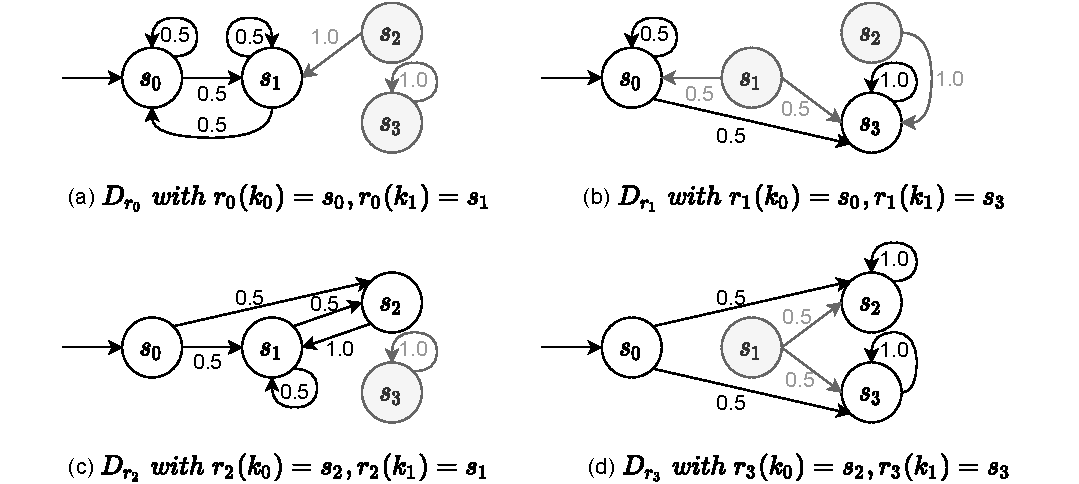
\includegraphics[width=0.9\textwidth]{figures/MCFamily.pdf}
\caption{A family $\fml$ of four various realisations. Unreachable states are greyed out.}%
\label{fig:mcfamily}%
\end{figure}

\textit{Quotient} MDP $M^\fml$ simulates the~behaviours of each member of the~family $\fml$ and can even pass between them during the~execution.
In more precise,~when the~path $s_0s_1s_2 \dots$ is executable in some family member $D_r$,~then it is also executable in $M^\fml$ as $s_0 \overset{r}{\rightarrow} s_1 \overset{r}{\rightarrow} \dots$.
However,~there may exist a~path $\pi$ that is executable in $M^\fml$,~but it is not realisable in neither of the~family members.
We can conclude that \textit{quotient} MDP over-approximates the~behaviours of the~members of family $\fml$.

\begin{definition}[Quotient MDP] \label{def:quotient_mdp}
\cite{roman-DP}
Let $\fml = \family$ be an~MCs family.
A~\textit{quotient} MDP $M^\fml$ of the~family $\fml$ is a~tuple $(S, s_{init}, \mathcal{R}^\fml, \mathcal{P})$,~where $\mathcal{P}(\cdot)(r) \equiv \mathcal{B}_r$.
\end{definition}

A~restriction of a~\textit{quotient} MDP concerning $\rlz \subseteq \rlz^\fml$ induces an~MDP which takes into account only transitions associated with $\rlz$.
We define the~usage of \textit{consistent} schedulers ensuring that execution of a~\textit{quotient} MDP always selects the~concrete realisation.
We note that a~\textit{consistent} scheduler yields a~specific family member for a~\textit{quotient} MDP,~which directly follows from Definition~\ref{def:quotient_mdp}.

\begin{definition}[Consistent scheduler]
\cite{roman-DP}
Let $\fml = \family$ be a~MCs family and let $M^\fml = (S, s_{init}, \mathcal{R}^\fml, \mathcal{P})$ be a quotient MDP of the~family $\fml$.
For $r \in \rlz^\fml$,~a (memory-less) scheduler $\sigma_r \in \sigma^{M^\fml}$ is called \textit{r-consistent} iff $\forall s \in S: \, \sigma(s) = r$.
A~scheduler is called \textit{consistent} iff it is consistent for some $r \in \rlz^\fml$.
\end{definition}

\subsection{Probabilistic Synthesis}
We use a~\textit{sketch}~\cite{sketching1,sygus}, ~which represents a~incomplete high-level description of a~probabilistic system,~to describe the~family of MCs.
It usually describes the~modelled system's fixed behaviour,~but it also contains the~undefined one represented by \textit{holes}.
They represent the~incomplete parts of a~program that must be instantiated so that the~final description satisfies a~given specification.
We note that the~holes correspond to parameters,~and their instantiation yields a~concrete Markov chain.
At follow, we formalise the sketch defining the set of designs:

\begin{definition}[Sketch]
Let $\sketch$ be a~sketch containing holes from the~set $\mathcal{H} = \left\{ H_k \right \}_k$ with $R_k$ being the~set of options available for hole $H_k$.
Let $\rlzf = \prod_k R_k$ denote the~set of all hole assignments (realizations),~$\sketch[r]$ denote the~program induced by a~substitution $r \in \rlzf$ and $\fmlr$ denote the underlying MC.
Note that the~set $\rlzf$ is exponential in $\lvert \mathcal{H} \rvert$.
\end{definition}

\todo{Some description ...}

\begin{definition}[Specification]
In our work,~we focus on the~conjunctions of specifications with \textit{reachability} and \textit{expected rewards}.
Let $T$ be a~set of target states,~then the~reachability property $\varphi \equiv \reachability{\bowtie}{\lambda}{T}$ where $\bowtie \in \{<, \leq, >, \geq\}$ and $0 \leq \lambda \leq 1$ expresses that the~probability of reaching $T$ refers to $\lambda \in [0,1]$ in agreement with $\bowtie$.
Expected reward property $\phi \equiv \reward {\bowtie}{\lambda}{T}$ expresses that the~expected reward accumulated before $T$ is reached refers to $\lambda \in \mathbb{R}^+$ in accordance with $\bowtie \, \in \{<, \leq \}$.
Let $\mathcal{P}[r]$ be a~program induced by the~realisation $r$,~we denote $\mathcal{P}[r] \models \varphi$ when this program satisfies the~specification $\varphi$.
Let $\varPhi = \{ \varphi_i \}_{i \in I}$ be a~finite set of specifications,~when $\forall i \in I: \mathcal{P}[r] \models \varphi_i$ then we write $\mathcal{P}[r] \models \varPhi$.
\end{definition}

We aim to two kinds of synthesis tasks for a~given probabilistic program described with a~realisation set $\rlzf$,~and a~specification set $\varPhi$.
The first task tries to identify just one realisation $r \in \rlzf$ that satisfy the~given specification set $\varPhi$.
This task represents a~special instance of the~threshold synthesis,~which tries to divide the~realisation set $\rlzf$ into two subsets based on their satisfiability.
We do not address this synthesis task in our work.
The second task on which we focus our attention is finding a~realisation that minimises or maximises a~given objective.

\begin{definition}[Feasibility]
Find a realisation $r \in \rlzf$ such that $\mathcal{P}[r] \models \varPhi$. 
\end{definition}

\begin{definition}[Minimality] \label{def:minimality}
For property $\phi_{\min}$, find a realisation $r^* \in \rlzf$ such that:
$$r^* \in \argmin_{r \in \rlzf} \left \{ \prob[\sketch[r] \models \phi_{\max}] \mid \sketch[r] \models \varPhi \right \}.$$.
\end{definition}

We defined only minimal synthesis task for probability property,~but its variants for maximisation and expected rewards may be defined analogously.
Moreover, we focus also to a relaxed variant of minimal synthesis, the so-called \textit{$\varepsilon$-minimal synthesis}, defined as follows: $\mathcal{P}[r^*] \models \varPhi \; and \; 
\mathbb{P}[\mathcal{P}[r^*] \models \varphi_{min}] \leq (1 - \varepsilon) \cdot \min_{r \in \mathcal{\overline{R}}} \{ \mathbb{P}[\mathcal{P}[r] \models \varphi_{min}] \; \lvert \; \mathcal{P}[r] \models \varPhi \}.$

\begin{example} (Synthesis problem)
Assume an~MCs family $\fml$ from Example~\ref{exam:mcfamily} and the~specification $\phi = \reachability{\geq}{0.1}{\{s_1\}}$.
The solution to the~feasibility synthesis problem is,~for example,~the~realisation $r_0$, since $D_{r_0}$ has a~probability of $\frac{2}{3}$ to reach state $s_1$.
For $\varPhi = [F \; \{s1\}]$,~the~solution to the~maximal synthesis problem on MCs family $\fml$ is the~realisation $r_2$,~as MC $D_{r_2}$ has a~probability equal to one to reach state $s_1$.
\end{example}

\section{Synthesis Methods}
Existing methods for a~probabilistic programs synthesis can be separated into two orthogonal classes.
The~first class involves complete methods that prove the~non-existence,~or potentially optimally,~of the~given probabilistic program.
On the~contrary,~incomplete methods handling various evolutionary techniques and intelligent search strategies form the~second one~\cite{spl2}.
However,~these incomplete methods cannot treat unfeasible and optimal synthesis problems compared to the~complete methods.
Therefore, we focus on the~complete state-of-the-art methods even though the~incomplete methods provide a~valuable flexibility level.
As a~reference and baseline method,~we consider a~\textit{one-by-one} approach that enumerates through each design space member~\cite{onebyone}.
An~explosion of the~design space renders this technique unfeasible for large families,~necessitating using advanced approaches utilising the~arbitrary structure of~the Markov chain family.

This thesis focuses on the~complete methods considered within the~\textit{oracle-guided} synthesis approach~\cite{oracle1,oracle2}.
The~control unit called \textit{learner} selects a~realisation $r$ from the~designs family and passes it to the~performing unit called \textit{oracle}.
This unit provides an~answer to whether realisation $r$ satisfies a given specification $\varPhi$.
Whenever it is not this case,~it provides supplementary information representing counterexample (CEGIS) or bounds from MC model checking (AR).
For purposes of this thesis, two various orthogonal oracles can be considered:
\begin{enumerate}[label=(\roman*)]
    \item \textbf{Inductive Oracle} (CE): It tries to infer the~declarations (counter-examples) about other family members by analysing individual realisation~\cite{cegis}.
    \item \textbf{Deductive Oracle} (AR): Abstraction refinement oracle considers more family members at once and then infers the consequences of these members' constructed aggregation~\cite{cegar}.
\end{enumerate}

\paragraph{Inductive Oracle.}
\textit{Counter-examples} represents a~concrete system execution violating a~given specification $\phi$.
When considering the~probabilistic model checking of Markov chains,~the~counter-examples represent paths set,~which have the~probabilities added to a~quantity that violates $\bowtie \lambda$.
When an~MC D violates the~given specification $\phi$ ($MC \; D \; \not\models \phi$),~a~ \textit{counter-example} provides diagnostic information related to the~states causing the~violation.
We consider the~counter-examples related to critical sub-systems:

\begin{definition}[Counter-example]
Let $D = \mc$ be an MC with $s_{\bot} \notin S$.
An MC $D \! \downarrow \! C = (S \cup \{ s_{\bot} \}, s_0, \mathbf{P}')$ induced by $C \subseteq S$ is sub-MC of MC $D$, where the transition probability matrix $\mathbf{P}'$ is defined as follows:
\begin{align*}
    \mathbf{P}'(s) = 
    \begin{cases}
        \mathbf{P}(S) \quad & if \; s \in C \\
        [ s_{\bot} \mapsto 1 ] \quad & \l otherwise.  
    \end{cases}
\end{align*}
For the~given specification $\reachability{\leq}{\lambda}{T}$,~when holds $D \! \downarrow \! C \not \models \reachability{\leq}{\lambda}{(T \cap (C \cup \{ s_0 \}))}$, then we call the~sub-system $D \! \downarrow \! C$ as a~\textit{counter-example} (CE).
\end{definition}

Let $D_r$ be an~MC that violates the~given specification $\phi$.
The inductive oracle constructs the critical sub-system $D_r \! \downarrow \! C$ to compute other realisations that also violate $\phi$.
Subsequently, it uses this constructed sub-system to infer a set called \textit{conflict} for $D_r$ and $\phi$.

\begin{definition}[Conflict] \label{def:conflict_set}
For MCs family $\fml = \family$,~and the~set $C \subseteq S$,~the~conflict set $K_C$ is given by $\bigcup_{s \in C} supp(\mathcal{B}(s))$ and consist of relevant parameters.
\end{definition}

\paragraph{Deductive Oracle.}
As we said above,~a~\textit{quotient} MDP over-approximates the~behaviours of each Markov chain in the~currently analysed family $\fml$.
The~\textit{deductive} oracle performs the~model checking of this MDP,~and it can yields the~following results.
We consider the~following specification against which is performed relevant model checking: $\reachability{\geq}{\lambda}{T}$.
The model checking itself returns the corresponding lower ($x_{min}$) and upper ($x_{max}$) bounds, as well as the minimising ($\sigma_{min}$) and maximising ($\sigma_{max}$) schedulers on the considered reachability probability.
When $x_{max} < \lambda$,~the~synthesis task is unfeasible since for each family member $r \in \rlz^\fml$ holds that $\mathcal{D}_r \not\models \phi$.
On the~contrary,~when $x_{min} >= \lambda$,~the~oracle can return an~arbitrary family member as a~solution to the~synthesis task since each satisfies $\phi$.
Last but not least,~when $x_{min} \leq \lambda \leq x_{max}$,~we cannot decide this case,~except when the~scheduler $\sigma_{max}$ is consistent.
Such scheduler represents the~valid member of the~analysed family with $x_{max} \geq \lambda$,~so it is a solution to the~synthesis task.
Otherwise,~when scheduler $\sigma_{max}$ is not consistent,~the~considered abstraction is too over-approximate,~and the~problem is undecided.

\begin{figure*}[h!]
\centering
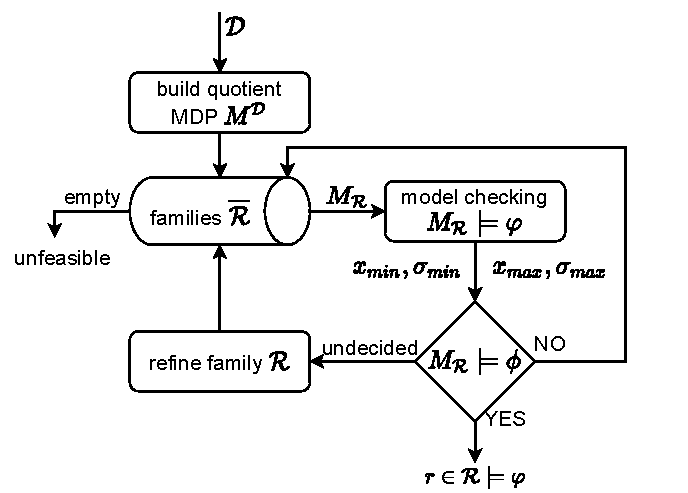
\includegraphics[width=0.70\textwidth]{figures/ar_loop.pdf}
\caption{An \textit{Abstraction Refinement} (AR) analysing loop.}%
\label{fig:architecture}%
\end{figure*}


In such a~case, we split the~undecidable family of Markov chains into two derived subfamilies. 
Then each of them represents the~input for deductive oracle,~which analyse them using the~technique introduced above.
When derived subfamilies are still undecidable, we refine them into smaller and smaller subfamilies until we find a~feasible solution or explore the~whole family.
When the~sub-family represents concrete realisation,~so it induces an~MC and not MDP ($x_{min} = x_{max}$),~such family is necessarily decided and have not split.
Moreover,~since the~family size is finite,~the~presented technique has guaranteed the~termination for these two reasons.
 
\paragraph{TODO NAME.} The~novel integrated approach,~the~so-called \textit{hybrid} method,~combines both these oracles and can thus take advantage of the~benefits offered by both approaches~\cite{roman-DP,tacas21}.
We illustrate the~cooperation between the~individual units within this method in Figure~\ref{fig:adaptivesynt}.
The~learner unit maintains the~subfamilies queue $\rlz' \subseteq \rlzf$ for subsequent processing and decides which oracle is selected based on their previous efficiency.
The~\textit{CE-Oracle} analyses the~family member $r$ and,~when it satisfies the~given specification $\varPhi$,~then returns it as a~solution.
On the~other hand,~it can generalise the~analysed realisation $r$ into a~subfamily $\rlz'$,~and the~learner unit can discard it from the~whole design space $\rlzf$.
Moreover,~this oracle exploits the~MDP bounds when constructing counterexamples,~thanks to which it can generate more petite generalisations.
The~\textit{Abstr-Oracle} analyses a~given sub-family $\rlz \subseteq \rlzf$,~and according to the~result,~it performs the~subsequent action.
When all realisations $r \in \rlz$ satisfy $\varPhi$,~then it returns the~overall synthesis result as feasible.
In another case,~when all realisations violate $\varPhi$,~the~whole analysed sub-family $\rlz$ will be discarded from the~families queue $\rlzf$ by the~learner.
The last option returns safe bounds on the best- and worst-case behaviour of all realisations in $\rlz$ considered $\varPhi$ when the analysis result is inconclusive.

\begin{figure}[ht!]
    \centering
     \begin{tikzpicture}
    \node[rectangle, draw, inner sep=8pt] (learner) {Learner};
    \node[rectangle, draw, inner sep=8pt,right=2.7cm of learner] (oracle) {CE-Oracle};
       \node[rectangle, draw, inner sep=8pt,left=2.7cm of learner] (abst) {Abstr-Oracle};
    \node[above=0.5cm of learner] (rlz) {$\rlzf$};
    \draw[->] (rlz) -- (learner);
    \node[above=0.5cm of oracle] (phi) {$\varPhi$};
    \draw[->] (phi) -- (oracle);
    \node[above=0.5cm of abst] (phiab) {$\varPhi$};
    \draw[->] (phiab) -- (abst);
    \draw[->] (learner) edge[bend left=10] node[above] {\scriptsize{$r \in \rlzf$}+bounds} (oracle);
    \draw[->] (oracle) edge[bend left=10] node[below] {\scriptsize{$\rlz' \subseteq \rlzf$ violate $\varPhi$}} (learner);
      \draw[->] (learner) edge[bend right=10] node[above] {\scriptsize{$\rlz \subseteq \rlzf$}} (abst);
    \draw[->] (abst) edge[bend right=10] node[below,align=center] {\scriptsize{bounds \emph{or} $\rlz$ violates}} (learner);
    
    \node[below=0.4cm of oracle] (sat) {$r \models \varPhi$};
    \draw[->] (oracle) -- (sat);
    \node[below=0.4cm of abst] (allsat) {each $r \in \rlz$, $r \models \varPhi$};
    \draw[->] (abst) -- (allsat);
    \node[below=0.4cm of learner] (unsat) {no $r \models \varPhi$};
    \draw[->] (learner) -- (unsat);
    \end{tikzpicture}
  \vspace{-0,5em}
    \caption{Oracle-guided synthesis (adapted from~\cite{tacas21}).}
    \label{fig:adaptivesynt}.
    \vspace{-1em}
\end{figure}

\paragraph{Hybrid Method.}
An~extended synthesis approach was introduced in~\cite{roman-DP,tacas21} using the~abstraction refinement to family prune and accelerating the~construction of counter-examples by CE-oracle.
Its main idea is to perform a~limited number of abstraction refinement loops and then invoke CEGIS to one of the~refined sub-families.
It turned out that a~moment of the~switching can be crucial,~and therefore,~the~method has to detect the~rightest moment.
One AR iteration is typically significantly slower than one CEGIS iteration since the~AR iteration involves an~MDP model-checking,~which inspires whole method workflow.
The~advance of the~hybrid methods is also constructing counter-examples within the~CEGIS loop,~where it uses a~fast greedy approach providing smaller generalisations.

\begin{algorithm}[H]
\hspace*{\algorithmicindent} \textbf{Input:} A MCs family $\fml$, a reachability property $\varphi$. \\
\hspace*{\algorithmicindent} \textbf{Output:} $Realization\; r \in \rlzf \; s.t. \; \mathcal{D}_r \models \varphi$, otherwise UNSAT. \\
\vspace*{-1.5em}
\begin{algorithmic}[1]
    \STATE $\rlzf \leftarrow \{ \rlz^{\fml} \}$ \hfill \textbf{// each analysed (sub)-family also holds bounds}
    \STATE $\delta_{CEGIS} \leftarrow 1$ \hfill \textbf{// time allocation factor for CEGIS}
    \WHILE{$\rlzf \neq \emptyset$}
        \STATE result, $\rlzf'$, $\sigma_{AR}$, $t_{AR}$ $\leftarrow$ AR($\rlzf$, $\varphi$)
        \IF{\textbf{satisfiable}(result)}
            \RETURN result
        \ELSE
            \STATE result, $\rlzf''$, $\sigma_{CEGIS}$ $\leftarrow$ CEGIS($\rlzf'$, $\varphi$)
            \IF{\textbf{satisfiable}(result)}
                \RETURN result
            \ELSE
                \STATE $\delta_{CEGIS}$ $\leftarrow$ $\sigma_{CEGIS}$ / $\sigma_{AR}$
                \STATE $\rlzf$ $\leftarrow$ $\rlzf''$
            \ENDIF
        \ENDIF
    \ENDWHILE
    \RETURN{UNSAT}
\end{algorithmic}
\caption{Hybrid method: Feasibility synthesis with single property.}
\label{alg:hybrid}
\end{algorithm}

As we said above,~this \textit{novel integrated} method combines inductive and deductive oracles,~and we briefly summarise their operation.
CEGIS iterates through all family members (realisations) until it reached the~satisfying realisation,~if such exists,~or when it explores the~whole design space.
Moreover,~it constructs counter-examples whenever the~analysed realisation $r \in \fmlr$ unsatisfying the~given specification $\varPhi$.
Realisations subset $\rlz' \subseteq \rlzf$ represents such counter-examples that CEGIS subsequently prunes from the~analysed design space $\rlzf$.
On the~other hand,~an AR loop builds MDP models from the~sub-families queue $\rlz \subseteq \rlzf$ that model-checkers analyse in follows.
When the~analysis results are inconclusive,~an AR refines the~analysed sub-family and  stores the~obtained satisfiability bounds for further processing within CEGIS loop.
Method allocates the~time per both loop according to their performance,~e.g.,~it can consider the~number of pruned MCs per timed unit and estimates an~efficiency from it.
Namely,~when it notices that AR prunes sub-families twice as slow as CEGIS,~it increases time twice in the~next round for CEGIS.
The resulting algorithm is summarised in Algorithm~\ref{alg:hybrid},~adapted from~\cite{tacas21}.


\chapter{Advanced Methods for Probabilistic Synthesis}\label{chap:advanced}
The~developed framework for \textit{integrated} synthesis has been designed for \textit{feasibility} synthesis concerning a~\textit{single} property.
However,~probabilistic programs often have to satisfy specifications expressed as a~\textit{conjunction} of several temporal logic constraints,~potentially including the~\textit{optimal} objective.
Therefore,~we design extensions to generalise the~\textit{hybrid} method to handle \textit{multi-property} specifications and treat \textit{optimal} synthesis.
In the~following,~we introduce these extensions to adapt the~integrated synthesis for both advanced methods. 
We design them individually for both \emph{CEGIS} and \emph{AR} loop,~whereas the overall framework of the~hybrid method is unchanged.

\section{Multi-Property Synthesis}
When considering \textit{multi-property} specifications,~the basic ideas of both oracles (\textit{CEGIS} and \textit{AR}) remain the~same.
When \textit{AR} analyses the quotient MDP concerning multiple properties, it yields multiple probability bounds.
\textit{CEGIS} loop constructs a~separate conflict for each unsatisfied property whenever it meets an~unsatisfiable realisation.
Moreover,~it uses the~corresponding probability bounds obtained at the~\textit{AR} loop to improve the quality of generated counter-examples.

\paragraph{CEGIS.}
The~CEGIS performs the~\textit{multi-property} synthesis in the~almost same manner as the~\textit{feasibility} synthesis for a~single property,~but there are a~few differences.
We decided to analyse each property $\varphi_i \in \varPhi$ for each considered realisation $r \in \rlz$,~even if we come across a~property that the~given realisation does not satisfy.
We construct the~counter-examples whenever the~analysed realisation $r$ does not satisfy the~given specification $\varphi_{i}$.
In this way,~we~prune the~design space of the~analysed family more efficiently because each constructed counter-example throws out a~certain number of family members.
The core of the loop stays the same.
We pick the~concrete realisation $r \in \rlz$,~then construct the~corresponding MC $\mathcal{D}_r$ and perform the~model checking against to current specification $\varphi_i$.
The~synthesis terminates when a~satisfying realisation against the~whole specification set $\varPhi$ is found,~or the~whole state space is exhausted,~indicating that no feasible solution in the~analysed family exists.


\begin{algorithm}[h!]
\hspace*{\algorithmicindent} \textbf{Input:} A family $\fml$ of MCs with the set $\rlz \subseteq \rlzf$ of realisations, and a set of properties $\varPhi = \{ \varphi_0, \dots, \varphi_{N-1} \}$. \\
\hspace*{\algorithmicindent} \textbf{Output:}  A realisation $r \in \rlz$ such that $\forall \; 0 \leq i < N. \; \mathcal{D}_r \models \varphi_i$, if such exists, otherwise $\mathtt{UNSAT}$. \\
\vspace*{-1.5em}
\begin{algorithmic}[1]
    \WHILE{$\rlz \neq \emptyset$}
        \STATE $\mathtt{allSat} \leftarrow \mathtt{True}$
        \STATE $r \leftarrow \mathtt{any(\rlz)}$
        \STATE $\mathcal{D}_r\leftarrow \mathtt{buildDTMC(\mathcal{R}, r)}$
        \FOR{$\varphi_i \in \varPhi$}
            \STATE $\mathtt{sat} \leftarrow \mathtt{solveDTMC(\mathcal{D}_r, \varphi_{i})}$
            \IF{$\mathtt{sat}$}
                \IF{$i = N - 1 \; \wedge \; \mathtt{allSat}$}
                    \RETURN $r$
                \ELSE
                    \STATE $\mathtt{continue}$
                \ENDIF
            \ELSE
                \STATE $\mathcal{R} \leftarrow \mathcal{R} \setminus \mathtt{constructCE}(\mathcal{D}_r, \varphi_{i})$
                \STATE $\mathtt{allSat} \leftarrow \mathtt{False}$
            \ENDIF
        \ENDFOR
    \ENDWHILE
    \RETURN $\mathtt{UNSAT}$
\end{algorithmic}
\caption{CEGIS loop: Multi-property synthesis.}
\label{alg:cegis_multi}
\end{algorithm}

\paragraph{Abstraction Refinement.}
\textit{Multi-properties} synthesis within the~AR loop is performed in the~same loop as the~single-property synthesis,~with some modifications.
The~algorithm's input represents the~MCs family $\fml = \family$ with the~corresponding set of realisations $\rlz \subseteq \rlzf$,~and a~set of properties $\varPhi_D$ explicitly determined for this family $\fml$.
This specification set $\varPhi_\fml$ includes the~specifications that need to be analyzed within the~family,~in other words,~specifications that have not yet been satisfied.

The~algorithm first constructs the~\textit{quotient} MDP $M^\fml$ concerning the~given family $\fml$ and realisation set $R$,~and then iterates over sub-families of $U$ that have not been yet analysed.
For each selected sub-family $\fml$ is then performed the~MDP model checking on the~relevant restricted MDP,~which yields computed minimal ($\mathtt{min}$) and maximal ($\mathtt{max}$) probabilities,~and corresponding schedulers ($\sigma_{min}$ and $\sigma_{max}$) related to them,~respectively.

\begin{algorithm}[h!]
\hspace*{\algorithmicindent} \textbf{Input:} A family $\fml$ of MCs with the set $\rlz \subseteq \rlzf$ of realisations, and a properties set $\varPhi_{\fml} = \{\varphi_0, \dots, \varphi_M \}$. \\
\hspace*{\algorithmicindent} \textbf{Output:}  A realisation $r \in \rlz$ s.t. $\forall \; 0 \leq i < M. \; \mathcal{D}_r \models \varphi_i$, if such exists, otherwise $\mathtt{UNSAT}$. \\
\vspace*{-1.5em}
\begin{algorithmic}[1]
    \STATE $U \leftarrow \{ \rlz \}$
    \STATE $M^\fml \leftarrow \mathtt{buildQuotientMDP(\fml, \rlz)}$ \hfill \textbf{// Applying Definition 7 and 8 in~\cite{cegar}}
    \WHILE{$U \neq \emptyset$}
        % \STATE $\mathtt{allSat} \leftarrow \mathtt{True}$
        \STATE $\mathtt{select \; \rlz \in U}$, and $U \leftarrow U \setminus \{ \rlz \}$
        \STATE $M^\fml[\rlz] \leftarrow \mathtt{restrict(M^\fml, \rlz)}$ \hfill \textbf{// Applying Definition 12 in~\cite{cegar}}
        \FOR{$\varphi_i \in \varPhi_\fml$}
            \STATE $\sigma_{min}, \ min \leftarrow \mathtt{solveMinMDP(M^\fml[\rlz], \varphi_{i})}$
            \STATE $\sigma_{max}, \ max \leftarrow \mathtt{solveMaxMDP(M^\fml[\rlz], \varphi_{i})}$
            \STATE $\mathtt{sat}, \; \sigma \leftarrow \mathtt{checkResult}(\mathtt{min}, \, \mathtt{max}, \, \varphi_i)$
            \IF{$\mathtt{sat}$}
                \STATE $\mathbf{if} \; i = M-1 \; \mathbf{then} \; \mathbf{return} \; \mathtt{any(\rlz)} \; \mathbf{else} \; \mathtt{continue}$
            \ENDIF
            \IF{$\neg \mathtt{sat}$}
                \STATE $\mathbf{break}$
            \ENDIF
            \IF{$\exists \; r \in \rlz. \; \mathtt{isConsistentScheduler(\sigma)}$}
                \RETURN $r$
            \ENDIF
            \STATE $U \leftarrow U \; \cup \; \mathtt{split(\rlz, min, max, \sigma_{min}, \sigma_{max})}$ \hfill \textbf{// A comprehensive info in~\cite{cegar}} 
        \ENDFOR
    \ENDWHILE
    \RETURN{$\mathtt{UNSAT}$}
\end{algorithmic}
\caption{AR loop: Multi-property synthesis.}
\label{alg:ar_multi}
\end{algorithm}

\section{Optimal Synthesis}
\textit{Optimal} synthesis is designed similarly to the~\textit{feasibility} synthesis,~with one significant difference.
An~\textit{optimising} property represents the~given \textit{optimal} property,~and its threshold is updated whenever satisfactory realisation is found.
The goal is to exclude this solution from the~searched state space.
For instance,~this update translates to decreasing the~threshold of the minimising property when the~\textit{minimal} synthesis considered.
The~optimal synthesis yield the~optimal solution when all family members were explored.

\paragraph{CEGIS.}
The~algorithm to perform the~\textit{CEGIS} loop for minimal synthesis takes as the~input a~family of MCs $\fml = \family$,~represented with realisations set $\rlz \subseteq \rlzf$,~and the~given minimisation specification $\varphi_{min}$.
This approach synthesises a~realisation $r^* \in \rlz$ minimising the~satisfaction probability $\mathtt{min^*}$ of the~given minimal objective.
Initially,~the~algorithm sets the~corresponding threshold of minimal objective concerning its settings and pick any realisation $r \in \rlz$.
Subsequently,~it builds the~corresponding Markov chain $\mathcal{D}_r$ and performs the~model checking against to given objective $\varphi_{min}$.

We then check whether $\mathcal{D}_r \models \varphi_{min}$ and when yes,~we moreover check whether the~obtained quantitative $\mathtt{result}$ is less than currently found minimum $\mathtt{min^*}$.
We update the~current optimal realisation $\mathtt{r^*}$ and corresponding minimal value $\mathtt{min^*}$ according to the~currently analysed realisation in such a~situation.
Moreover,~we update the~threshold of the~\textit{minimising} property represented the~given minimal objective according to the~newest one.
We do this to not analyse for realisations worse than the~current one in subsequent iterations but to prune them by constructing counter-examples.

Otherwise,~when $\mathcal{D}_r \not\models \varPhi_{min}$ or the~current result is not better than the~current minimum,~we compute a~critical set $C$ for $\mathcal{D}_r$ and $\varphi_{min}$.
This critical set $C$ represents a~fragment of the~whole state space $S$ of the~analysed family $\fml$.
Subsequently,~the algorithm~constructs the~sub-system $\mathcal{D}\!\downarrow\!C$ as a~counter-example concerning computed critical set $C$.
We then subtract these constructed counter-examples from the~set $\fml$ of candidate solutions. 
We repeat this procedure until either the~whole state space is exhausted and at the~end returns the~found minimising realisation $\mathtt{r^*}$ and corresponding value $\mathtt{min^*}$.
This approach is summarised in Algorithm~\ref{alg:ar_optimal}.

\begin{algorithm}[h!]
\hspace*{\algorithmicindent} \textbf{Input:} A family $\fml$ of MCs with the set $\rlz \subseteq \rlzf$ of realisations, and a property $\varphi_{min}$. \\
\hspace*{\algorithmicindent} \textbf{Output:}  A realisation $r^* \in \rlz$ according to Definition~\ref{def:minimality}. \\
\vspace*{-1.5em}
\begin{algorithmic}[1]
    \STATE $\mathtt{min^*} \leftarrow 0$, $\mathtt{r^*} \leftarrow \emptyset$
    \STATE $\varphi_{min} \leftarrow \mathtt{setThreshold(min^*)}$
    \WHILE{$\rlz \neq \emptyset$}
        \STATE $r \leftarrow \mathtt{any(\rlz)}$
        \STATE $\mathcal{D}_r\leftarrow \mathtt{buildDTMC(\mathcal{R}, r)}$
        \STATE $result \leftarrow \mathtt{solveDTMC(\mathcal{D}_r, \varphi_{min})}$
        \IF{$result < min^*$}
            \STATE $\mathtt{r^*} \leftarrow r$, $\mathtt{min^*} \leftarrow min$
            \STATE $\varphi_{min} \leftarrow \mathtt{setThreshold(min^* - min^* \cdot \varepsilon)}$
        \ELSE
            \STATE $\mathcal{R} \leftarrow \mathcal{R} \setminus \mathtt{constructCE}(\mathcal{D}_r, \varphi_{min})$
        \ENDIF
    \ENDWHILE
    \RETURN $r*$, $min^*$
\end{algorithmic}
\caption{CEGIS loop: Minimality synthesis.}
\label{alg:cegis_optimal}
\end{algorithm}

\paragraph{Abstraction Refinement.}
We illustrate the~\textit{minimality} synthesis process within the AR loop by Algorithm~\ref{alg:ar_optimal}.
We remind that the~synthesis target is to find realisation $r^* \in \rlzf$ that minimises the~satisfaction probability $\mathtt{min^*}$ of the~minimal objective.
A~set $U$ serves to store sub-families of the~given family of realisations $\rlz$ that have not been yet analysed.
The~algorithm starts with building the~quotient MDP for the~whole analysed family $\fml$ concerning the~current realisations set $\rlz \subseteq \rlzf$.
Subsequently,~it restricts the~set of realisations to obtain the~corresponding sub-family for every $\rlz \in U$,~concerning the~quotient MDP $M^\fml$. 
Then,~the~algorithm continues with running the standard MDP model checking to compute the~minimal and maximal probability and corresponding schedulers,~respectively.

The~main difference between the~AR loop when feasibility synthesis is performed and now is the~interpretation of the~underlying MDP model checking results.
The~algorithm can discard $\rlz$ when the~$\mathtt{min}$ probability for $\rlz$ is above $\mathtt{min^*}$.
Otherwise,~it is required to check whether the~corresponding scheduler $\sigma_{min}$ is \textit{consistent} or not.
When it is consistent,~we can discard $\rlz$ and updated the current $\mathtt{min^*}$ and $\sigma_{min}$, respectively.
When the scheduler is not consistent but $\mathtt{max < min^*}$ is valid,~we can still update the~current $\mathtt{min^*}$ and enhance the~pruning process.
In such a~situation,~some realisations in $\rlz$ induce a~lower probability than current $\mathtt{min^*}$,~but actually,~we do not know which ones.
However,~when the~scheduler is not consistent,~regardless of whether $\mathtt{min^*}$ has been updated,~the~algorithm has to split the~analysed realisations set $\rlz$.
Consequently,~the~algorithm subsequently has to analyse the~derive sub-families since they can cover the~minimising realisation.

Whenever the~set $U$ is empty,~so all sub-families have been analysed,~the~algorithm terminates and yields the~found optimal realisation $r^*$.
This realisation is obtained by applying the~function \texttt{applyScheduler} concerning Definition~\ref{def:incuded_mc}.
The~termination is guaranteed since only a~finite number of subfamilies realisations has to be analysed.
We summarise this procedure in Algorithm~\ref{alg:ar_optimal}.

\begin{algorithm}[h!]
\hspace*{\algorithmicindent} \textbf{Input:} A family $\fml$ of MCs with the set $\rlz \subseteq \rlzf$ of realisations, and a property $\varphi_{min}$. \\
\hspace*{\algorithmicindent} \textbf{Output:}  A realisation $r^* \in \rlz$ according to Definition~\ref{def:minimality}. \\
\vspace*{-1.5em}
\begin{algorithmic}[1]
    \STATE $min^* \leftarrow 0$, $U \leftarrow \{ \rlz \}$
    \STATE $M^\fml \leftarrow \mathtt{buildQuotientMDP(\fml, \rlz)}$ \hfill \textbf{// Applying Definition 7 and 8 in~\cite{cegar}}
    \WHILE{$U \neq \emptyset$}
        \STATE $\mathtt{select \; \rlz \in U}$, and $U \leftarrow U \setminus \{ \rlz \}$
        \STATE $M^\fml[\rlz] \leftarrow \mathtt{restrict(M^\fml, \rlz)}$ \hfill \textbf{// Applying Definition 12 in~\cite{cegar}}
        \STATE $\sigma_{min}, \ min \leftarrow \mathtt{solveMinMDP(M^\fml[\rlz], \varphi_{min})}$
        \STATE $\sigma_{max}, \ max \leftarrow \mathtt{solveMaxMDP(M^\fml[\rlz], \varphi_{min})}$
        \IF{$min < min^*$}
% \hfill \textbf{// Applying Definition 10 in~\cite{cegar}}
            \IF{$\mathtt{isConsistentScheduler(\sigma_{min})}$}  
                \STATE $\sigma^* \leftarrow \sigma_{min}$, $min^* \leftarrow min$
            \ELSE
                \IF{$max < min^*$}
                    \STATE $min^* \leftarrow min$
                \ENDIF
                \STATE $U \leftarrow U \; \cup \; \mathtt{split(\rlz, min, max, \sigma_{min}, \sigma_{max})}$ \hfill \textbf{// A comprehensive info in~\cite{cegar}}
            \ENDIF
        \ENDIF
    \ENDWHILE
    \RETURN{$\mathtt{applyScheduler(\rlz, \sigma^*)}$}
\end{algorithmic}
\caption{AR loop: Minimality synthesis.}
\label{alg:ar_optimal}
\end{algorithm}


\chapter{Combined Probabilistic Synthesis}\label{chap:combined}


\chapter{\toolname{}}\label{chap:paynt}

\toolname{}\footnote{\url{https://github.com/gargantophob/synthesis}} (\underline{P}robabilistic progr\underline{A}m s\underline{YNT}hesiser) is a~tool to synthesise probabilistic programs automatically.
\toolname{} supports the~synthesis of finite-state programs and the~specifications given as a~conjunction of temporal logic constraints,~possibly including an~optimal objective.
The input is a~program sketch that concisely describes a~finite family of (finite) Markov chains,~and a~specification.
The tool can then identify a~family member that (potentially optimally) satisfies given specifications.
Figure~\ref{fig:sketching} depicts the workflow of \toolname{}.

\begin{figure*}[h!]
\centering
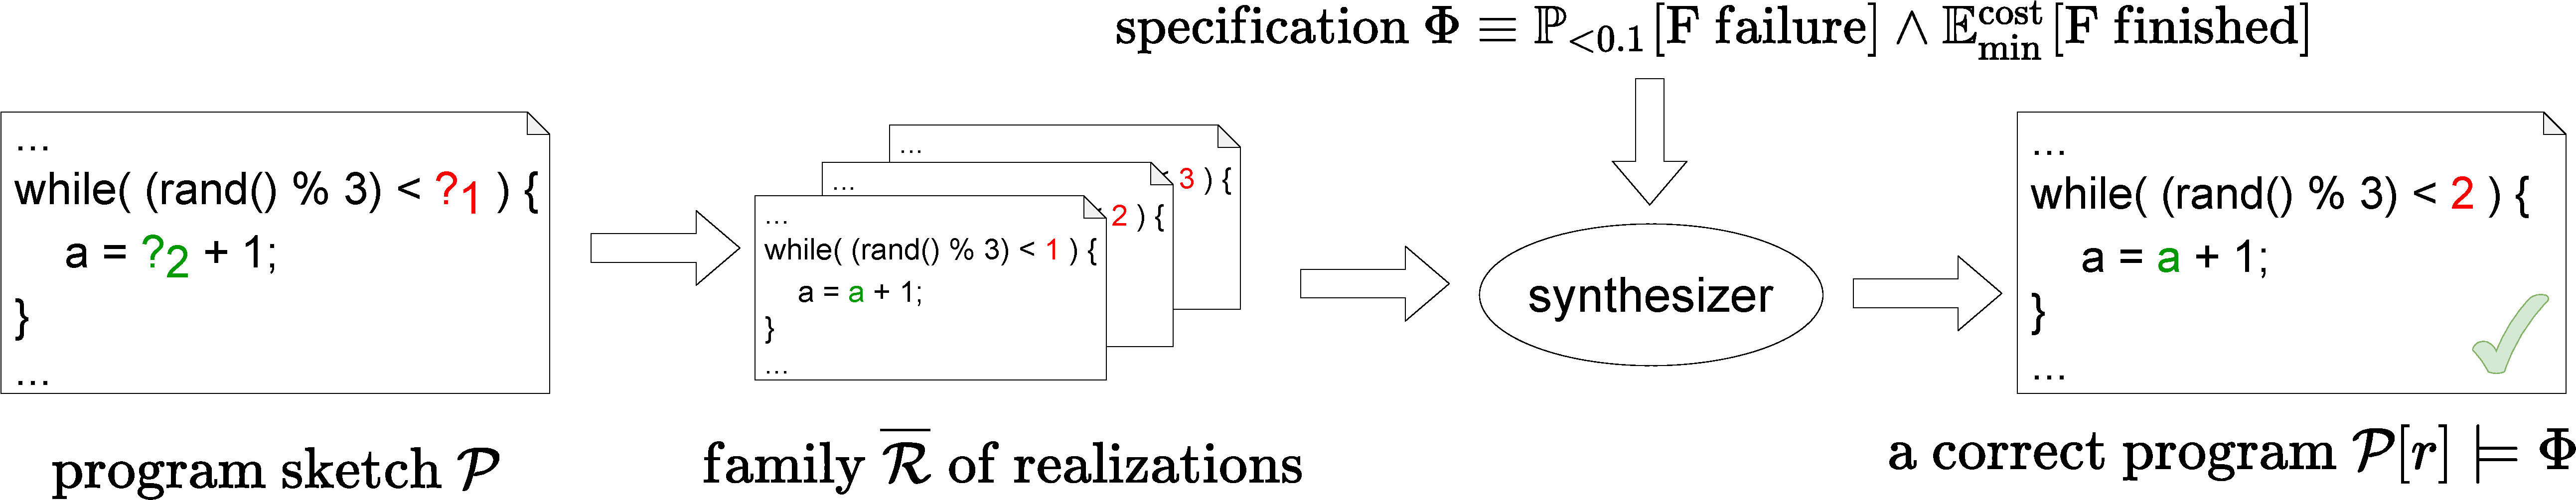
\includegraphics[width=1.0\textwidth]{figures/sketching}
\caption{The workflow of the synthesis process within \toolname{}.}%
\label{fig:sketching}%
\end{figure*}

\section{Architecture}

The design of \toolname{} is based on an~oracle-guided synthesis~\cite{tacas21} enabling a~flexible combination and integration of a~variety of state-of-the-art synthesis and verification algorithms. 
In particular,~it implements a~hybrid synthesis approach leveraging both the~\emph{CEGIS} and the~\emph{AR} oracle. 
\toolname{} is able to efficiently synthesise the~program topology (\emph{topology} synthesis) as well as continuous parameters affecting the~transition probabilities (\emph{parameter} synthesis).
Moreover,~it can handle sketches including both types of synthesis problems,~so-called a~\emph{combined} synthesis,~which is a~unique feature compering to the~existing tools. 

To achieve a high-performance synthesis, \toolname{} is implemented on top of the~probabilistic model chec\-ker \storm{}~\cite{STORM},~providing optimised verification procedures.
It is implemented in a~modular fashion on top of a~python API to provide flexibility.
\toolname{} allows to define of the~program sketches and provides all baseline synthesis algorithms under one roof.
The~tool finds application primarily for two groups of users.
First,~the~analysis of realisations sets is a~useful back-end for automated system design. %automatic engines.
For instance,~this can be used when synthesising finite-state controllers for partially observable Markov decision processes (POMDPs),~synthesising a~network protocol to increase the~packet throughput,~or selecting the~optimal power management strategy.
Second,~\toolname{} provides a modular development platform for automated design of probabilistic programs.

\begin{figure*}[h!]
\centering
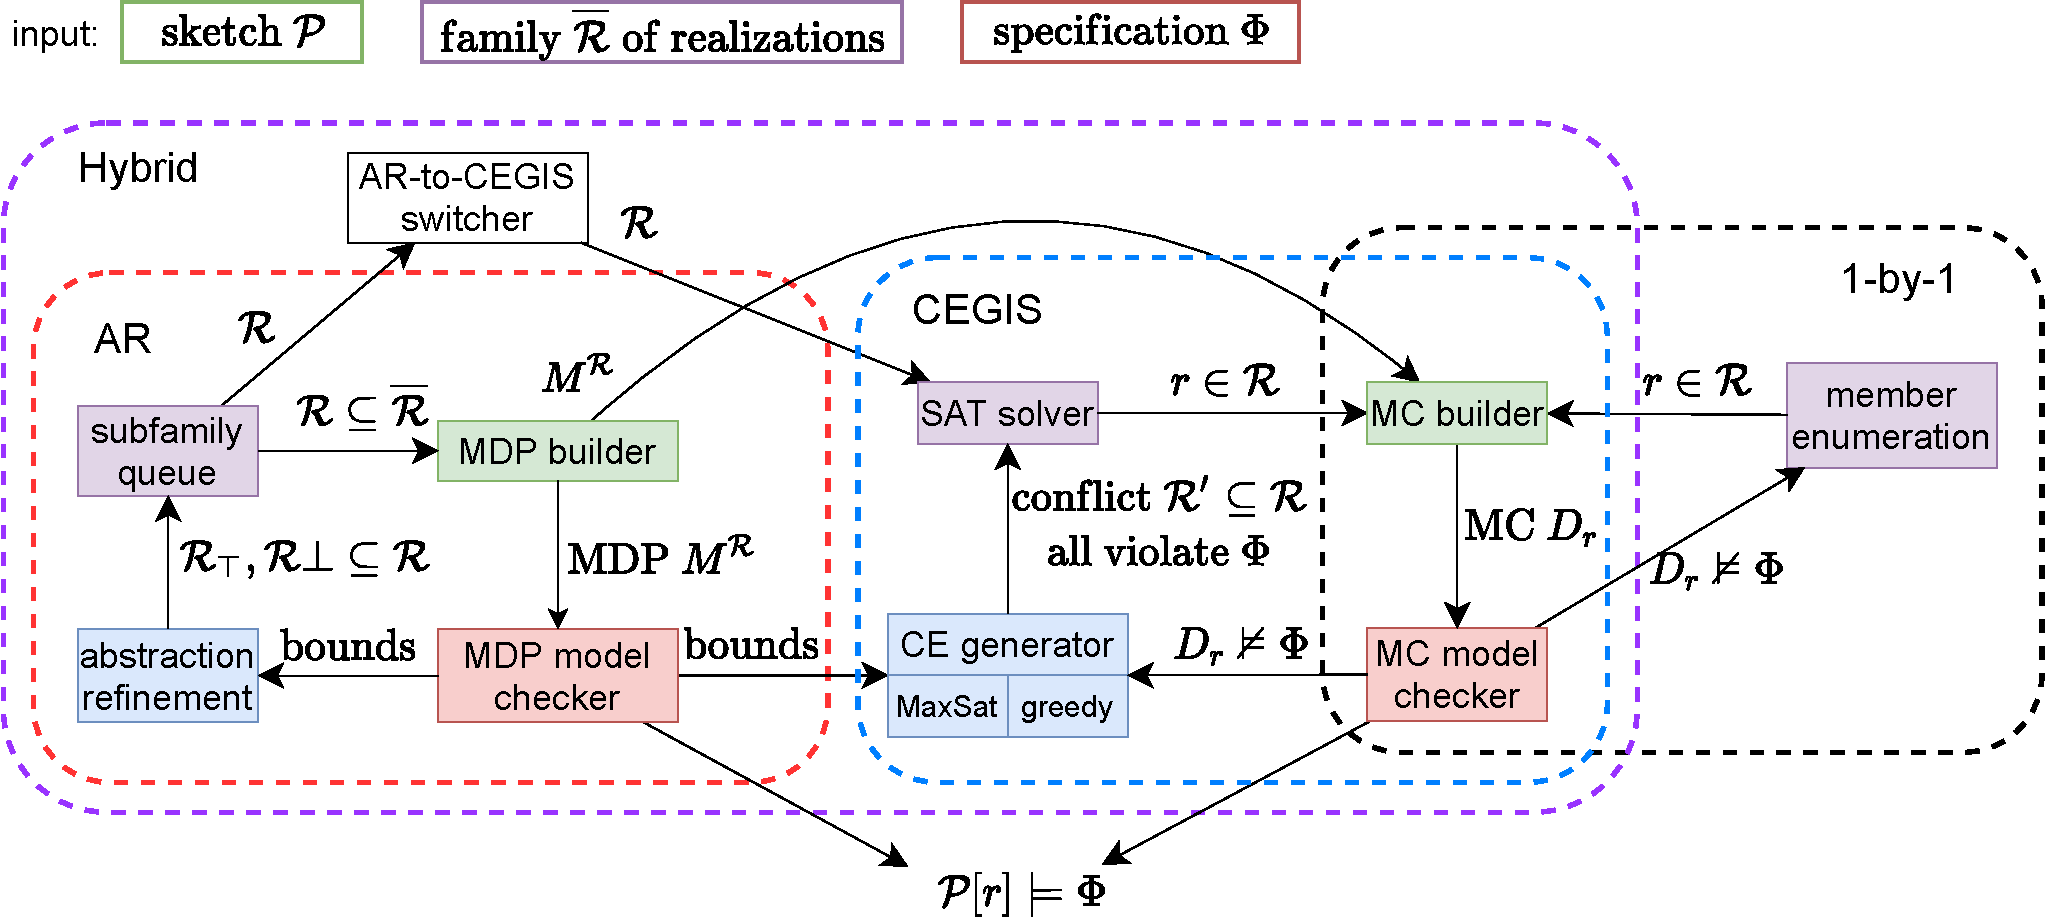
\includegraphics[width=1.0\textwidth]{figures/architecture.pdf}
\caption{The architecture of tool \toolname{}.}%
\label{fig:architecture}%
\end{figure*}

\toolname{}'s architecture (see Figure~\ref{fig:architecture}) consists of model checkers,~modules to build models and components for family handling.
The~family handlers store the~information about the~already covered design space of the~analysed family.
As the~name suggests,~the~member enumeration unit iterates over all family members.
SAT solver maintains an~SAT-formula describing undiscovered realisations,~and subsequent,~it uses Z3 SMT-solver to obtain the next candidate realisation.
The~queue with sub-families contains a~collection of unexplored sub-families refined as hyper-rectangles when the~analysis is inconclusive.
The~model builders take a~specific input according to the~active oracle and produce the~relevant model representation:
the~CE-oracle sends to the builder a single realisation $r$ while 
the~AR-oracle sends a~realisations set $\rlz' \subseteq \rlz$.
The~model checkers verify whether the constructed model (MCs or MDPs) satisfies the~given specification.
When analysing MDP,~lower and upper bounds on satisfiability probabilities are provided.
Last but not least,~\toolname{} provides a~module for generating counterexamples. In particular,~it implements two approaches: a~greedy state-expansion and a~MaxSat approach.

\paragraph{Implementation Frame.}
\toolname{} takes as the~input a~sketch written in the~\jani{} or \prism{} language and a~set of temporal properties expressed using the~PRISM syntax. 
\toolname{} is implemented on top of a~modern probabilistic model checker \storm{}~\cite{STORM} providing  high-performance verification procedures implemented in C++.
Further,~it uses Z3 theorem prover for SMT-solving and~a Python API for flexible implementation of the~synthesis loop itself.
The~implementation of \toolname{} is composed of \textit{30} Python modules containing \textit{7k} source lines of code.
We consider only our implementation and do not include extensions contributed to \storm{} and its Python API,~invoked by \toolname{}.
We tests the specific components with unit tests to maintain their correct functionality.
Regression tests verify the~accuracy and correctness of the~synthesis results and these tests currently cover more than \textit{90\%} of the~source code lines.

\section{\prism{} Sketch Language}
As we said above,~\toolname{} takes as the~input the~sketch written in the~\prism{}~\cite{KNP11} or \jani{}~\cite{jani} language.
These high-level programming languages to describe probabilistic systems are more advantageous than modelling the~system as a~Markov Chain.
The~state explosion problem,~arising when using the~Markov chains as an~operational model,~renders this approach unusable.
\storm{} parses the~high-level description (sketch) written in these languages and constructs the~corresponding Markov chain,~which the~individual synthesis methods analyse.
Now,~we briefly introduce the~\prism{} sketching language proposed in~\cite{cegis}.

A~program written in \prism{} language consists of modules that interact with between itself.
We consider only programs with a~single module since more modules can be transformed into one model program.
A~module state space is given by the~set of (bounded) variables,~with their initial values and the~set of guarded commands describing the~transitions between module states.
The commands have the following form:
\begin{align*}
\texttt{[action]} \
\texttt{guard}
\ \ \rightarrow \ \
p_1 : \texttt{update}_1 + \dots + p_n : \texttt{update}_n 
\end{align*}
The~\emph{actions} ensure the~synchronisation between two or more modules when they perform the~command.
The~\emph{guard} represents a~boolean expression over the~module variables.
An~update of the~variables is selected concerning the~probability distribution defined by expressions $p_1$ through $p_n$ when guard evaluates to true.
Essentially,~the guard identifies states for which this command is applicable,~and updates describe successor states and the~probability distribution over these successors.
Overlapping of guards is disallowed since it yields non-determinism.

Moreover,~a~\textit{sketch} describes a~program containing holes representing undefined program parts that should be filled with the~value from the~finite options set.
These holes are declared as follows:
\begin{align*}
    \texttt{type} \ \texttt{hole} \ \textit{h} \ \texttt{in} \ \ \{ \mathtt{expr_1}, \dots, \mathtt{expr_k} \}
\end{align*}
The~\texttt{type} represents the domain of \texttt{hole} \textit{h} and it is an \texttt{integer} or \texttt{float}.
The~hole identifier is given by \textit{h},~and the~set of expressions $\mathtt{expr_i}$ is defined over the~program variables.
Commands and variable declarations use a~\texttt{hole} as a~component of an~\texttt{update expression} or a~\texttt{guard}.
Such a~program sketch represents a~system description with a~specified general structure but with some concrete details left out.
Instantiating all holes yields a~specific program,~and the~synthesiser target is to resolve how to substitute all holes with their options to satisfy a~given specification.
\prism{} sketching language also provides several extra functionalities: specification of the~constraints to hole values and assigning costs to option holes,~and many others.
For more detailed information,~please refer to~\cite{cegis}.

\begin{example}[\prism{} Program]
For instance,~we introduce the~following \prism{} program $\sketch$:
\begin{align*}
    & \texttt{int} \ \texttt{hole} \ \mathit{X} \ \texttt{in} \ \{ 0,1 \} \\
    & \texttt{int} \ \texttt{hole} \ \mathit{Y} \ \texttt{in} \ \{ 1,2,3 \} \\
    & \texttt{module m} \\
    & \quad \texttt{int} \ \texttt{s:} \; [0..4] \; \texttt{init} \ \texttt{X+1} \\
    & \quad [] \ \texttt{s < Y} \ \rightarrow \ \texttt{0.75}: \ \texttt{(s' = max(s-X, 0))} \ \texttt{+} \ \texttt{0.25}: \ \texttt{(s' = s+X)}; \\
    & \quad [] \ \texttt{s = Y} \ \rightarrow \ \texttt{0.50}: \ \texttt{(s' = s-1)} \ \texttt{+} \ \texttt{0.50}: \ \texttt{(s' = s+1)}; \\
    & \quad [] \ \texttt{s > Y} \ \rightarrow \ \texttt{0.25}: \ \texttt{(s' = s-1)} \ \texttt{+} \ \texttt{0.75}: \ \texttt{(s' = min(s+1, 4))};  \\
    & \texttt{end module}
\end{align*}
\label{exa:prism}
\end{example}
The~module \texttt{m} can be in one of five states: $\{ 0,1,2,3,4 \}$.
When the~module state \texttt{s} is equal to the~value of hole \texttt{Y} (\texttt{s = Y}),~it will move to the~nearest previous (\texttt{s' = s-1}) or next (\texttt{s' = s+1}) state with the~same probability of \texttt{0.50}.
When the~module state \texttt{s} is above the~value of hole \texttt{Y} (\texttt{s > Y}),~it will move to the~left neighbour with the~probability of \texttt{0.75} and with remaining to the~right if it exists,~or stay in the~last state (\texttt{s=4}).
Otherwise (\texttt{s < Y}),~the model will move the~same as in the~previous case (\texttt{X=1}),~or it stays in the~current state without change (\texttt{X=0}).
When we consider the~following instantiating of the~holes \texttt{X=1} and \texttt{Y=2},~the~corresponding underlying Markov chain is depicted below.

\begin{figure*}[h!]
\centering
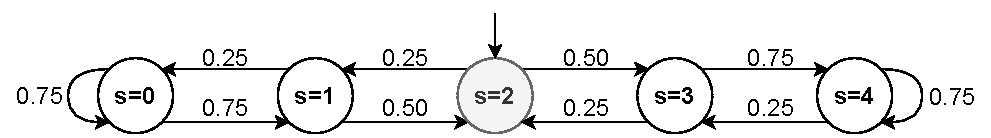
\includegraphics[width=1.0\textwidth]{figures/prism_dtmc.pdf}
\caption{An underlying Markov Chain of a probabilistic program $\sketch$ from Example~\ref{exa:prism}.}%
\label{fig:architecture}%
\end{figure*}

\section{Usage of \toolname{}}
We demonstrate the~usage of \toolname{} on a~synthesis problem considering a simple server for request processing depicted in Figure~\ref{fig:dpm}. 
Requests are produced by an~external unit within random intervals and maintained in a~request queue with capacity $Q_{max}$.
If the~queue is full arriving requests are lost.
The~server can operate in three modes having a different power consumption \,--\, \textit{active},~\textit{idle} and \textit{sleeping}.
The~server process the~requests only in the~\textit{active} state.
When the~server switches from a~state with low energy into a~state with higher,~extra energy is consumed,~and random latency is required.
We note that the~power consumption of request processing depends on the~current size of the~queue.
The~server operation time is finite but given as a~random process.

\begin{figure*}[h!]
\centering
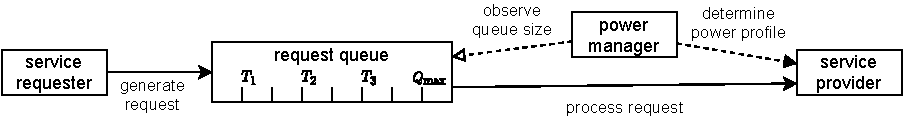
\includegraphics[width=0.9\textwidth]{figures/dpm.pdf}
\caption{The server for request processing within \emph{DPM} case study.}%
\label{fig:dpm}%
\end{figure*}

The~synthesis aims to construct a~unit called \textit{power manager} (PM),~which controls the~server.
PM observes the~current queue size and,~according to it,~then sets the~relevant power profile.
Precisely,~it differentiates between four queue occupancy levels determined by the~threshold levels $T_1,T_2$,~and $T_3$.
They indicate which fraction of the~queue capacity is currently occupied,~and they are entered into the~model as unknown parameters.
Since the~model considers three levels,~then the~power manager observers the~queue occupancy on the~following intervals: $\left[0, T_1 \right]$, $\left(T_1, T_2 \right]$, $\left(T_2, T_3 \right]$, $\left(T_3, 1 \right)$.
Moreover,~it considers a~single power profile $P_1,\dots,P_4 \in \{0,1,2\}$ for each occupancy level.
The~power profile's current value represents the~server's mode,~so the set~$\{0,1,2\}$ encodes available modes sleeping,~idle and active in the~given order.
The~following sketch describes the~module of \textit{PM}:

\begin{verbatim}
module PM
    pm  :  [0..2] init 0; // 0 - sleep, 1 - idle, 2 - active
    [sync0] q <= T1*QMAX -> (pm'=P1);
    [sync0] q > T1*QMAX & q <= T2*QMAX -> (pm'=P2);
    [sync0] q > T2*QMAX & q <= T3*QMAX -> (pm'=P3);
    [sync0] q > T3*QMAX -> (pm'=P4);
endmodule
\end{verbatim}

In this model,~we consider the~following parameters and their domains: the~queue capacity $Q_{\max} \in \{1,2,\dots,10\}$,~the~power profiles $P_1,\dots,P_4 \in \{0,1,2\}$ and the~thresholds $T_1 \in \{0.0,0.1,0.2,0.3,0.4\}$,~$T_2 \in \{0.5\}$,~$T_3 \in \{0.6,0.7,0.8,0.9\}$.
The~final sketch describing this considered model forms a~design space of $16,200$ various power managers.
The~average size of the Markov chains in this models is around $900$ states.
The~synthesis target is to find the~specific power manager,~i.e.,~the~holes instantiation,~that minimises power consumption while the~expected number of lost requests during the~server's operation time is below $1$.
We can formalise these requirements as a~pair of temporal logic formulae in the~\prism{} language:
\begin{verbatim}
R{"lost"} <= 1 [ F "finished" ]  
R{"power"}min=? [ F "finished" ]
\end{verbatim}

\toolname{} explores the~design space and produces the~following output,~including the~parameter assignment,~and the~quality value corresponds to $\Phi$ of the~analysed program:
\begin{verbatim}
QMAX=5,T1=0,T3=0.7,P1=1,P2=2,P3=2,P4=2
R[exp]{"lost"}=0.6823 [F "finished"]
R[exp]{"power"}min=9100 [F "finished"]
\end{verbatim}
The~synthesised power manager,~optimal wrt. to the~specified properties,~has the~queue capacity set to $5$ and individual thresholds at values  $1 = 0.0$, $2 = \floor{ 5\cdot 0.5}$ and $3 = \floor{ 5\cdot 0.7}$.
The~synthesised power manager performs the following strategy.
When the~request queue is empty,~then the~power manager maintains an~idle state.
Otherwise,~it always maintains an~active state,~regardless of the~exact size of the~queue,~and is never in the~sleeping state.
The~synthesised solution has a~power consumption of $9,100$ units and the~expected number of lost requests of $\approx 0.68 < 1$.

\toolname{} computes an~optimal solution in one minute. 
Although this synthesis problem is quite simple (recall it includes only 16k candidates),~\toolname{} is already $3 \times$ faster than a~naive enumeration of all realisations.
Further,~we explored a~more complex variant of this problem inspired by a~dynamical power manager's known model for complex electronic systems.
The~synthesis problem is described by the~sketch,~which covers a~family around 43M realisations.
\toolname{} solves this synthesis problem within 10~hours,~whereas the~naive enumeration takes more than one~month.

\chapter{Experimental Evaluation}\label{chap:experiments}


\chapter{Final Considerations}\label{chap:conclusion}


\section{Future Research}
\section{Conclusions}